\documentclass{article}
\usepackage{siunitx}
\usepackage{setspace}
\usepackage{gensymb}          
\usepackage{xcolor}
\usepackage{caption}
%\usepackage{subcaption}
%\doublespacing               
\singlespacing   
\usepackage[none]{hyphenat}   
\usepackage{amssymb} 
%\usepackage{relsize} 
\usepackage[cmex10]{amsmath}  
\usepackage{mathtools}      
\usepackage{amsmath}   
\usepackage{commath}  
%\usepackage{amsthm}    
%\interdisplaylinepenalty=2500 
%\savesymbol{iint}   
%\usepackage{txfonts}
%\restoresymbol{TXF}{iint}  
%\usepackage{wasysym}    
\usepackage{amsthm}   
\usepackage{mathrsfs}
\usepackage{txfonts}
\let\vec\mathbf{}
%\usepackage{stfloats}
\usepackage{float}
\usepackage{cite}
\usepackage{cases}
\usepackage{subfig}
%\usepackage{xtab}
\usepackage{longtable}
\usepackage{multirow}
%\usepackage{algorithm}
\usepackage{amssymb}
%\usepackage{algpseudocode}
\usepackage{enumitem}
\usepackage{mathtools}
%\usepackage{eenrc}
%\usepackage[framemethod=tikz]{mdframed}
\usepackage{listings}
\usepackage{listings}         
\usepackage[latin1]{inputenc}   
%% \usepackage{color}        
%% \usepackage{lscape}       
\usepackage{titling}                 
%\usepackage{fulbigskip}   
\usepackage{tikz}      
\usepackage{graphicx}
\graphicspath{{/Internal storage/Download/FWC
}}
\usepackage{atbegshi}
%http://ctan.org/pkg/atbegshi
\AtBeginDocument{\AtBeginShipoutNext{\AtBeginShipoutDiscard}}
\newcommand{\mydet}[1]{\ensuremath{\begin{vmatrix}#1\end{vmatrix}}}
\providecommand{\brak}[1]{\ensuremath{\left(#1\right)}}
\newcommand{\solution}{\noindent \textbf{Solution: }}
\newcommand{\myvec}[1]{\ensuremath{\begin{pmatrix}#1\end{pmatrix}}}
\let\vec\mathbf

\begin{document}
\begin{center}
\title{ALGEBRA}
\date{}
\maketitle
\end{center}
\begin{enumerate}

    \item What is the area of a semi-circle of diameter $'d'$?
    
    \begin{enumerate}
        \item $\frac{1}{16}\pi d^2$ \item $\frac{1}{4}\pi d^2$ \item $\frac{1}{8}\pi d^2$ \item $\frac{1}{2}\pi d^2$
    \end{enumerate}

    \item if one zero of the polynomial  \begin{align} p(x)=6x^2+37x-(k-2) \end{align} is reciprocal of the other, then what is the value of $k$?
    \begin{enumerate}
        \item $-4$ \item $-6$ \item $6$ \item $4$
    \end{enumerate}
    \item The zeroes of the polynomial \begin{align} p(x)=x^2+4x+3 \end{align} are given by:
    \begin{enumerate}
        \item $1,3$ \item $-1,3$ \item $1,-3$ \item $-1,-3$
    \end{enumerate}
    \item $sin\theta + cos\theta = \sqrt{3}$, then find the value of $sin\theta.cos\theta$.
    \item if $sin\alpha = \frac{1}{\sqrt{2}}$ and $cot\beta = \sqrt{3}$, then find the value of $cosec\alpha + cosec\beta$.
    \item Prove that:\begin{align}
    \frac{tan\theta+sec\theta-1}{tan\theta-sec\theta+1}=\frac{1+sin\theta}{cos\theta}
    \end{align}
    \item While designing the school year book, a teacher asked the student that the length and width of a particular photo is increased by $x$ units each to double the area of the photo. The original photo is $18 cm$ long and $12 cm$ wide.refer the given \figref{fig:figure1}
    Based on the above information, answer the following questions:
    \begin{enumerate}
        \item Write an algebraic equation depicting the above information.
        \item Write the corresponding quadratic equation in standard form.
        \item What should be the new dimensions of the enlarged photo?
    \end{enumerate}
    \begin{figure}[H]
        \centering
        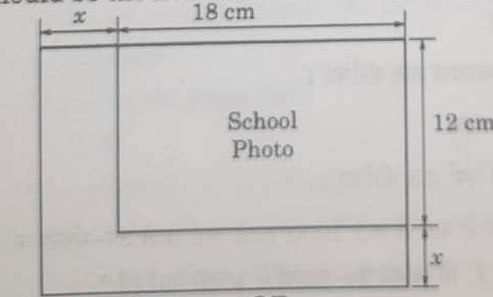
\includegraphics{figs/school.jpg}
        \caption{}
        \label{fig:figure1}
    \end{figure}
    \item Can any rational value of $x$ make the new area equal to $220 cm^2$?
\end{enumerate}
\end{document}
